% WEA 2026 Paper - Rule Base Sensitivity Analysis for Fuzzy PSO
% CCIS/LNCS format - Springer
%
\documentclass[runningheads]{llncs}
%
\usepackage[T1]{fontenc}
\usepackage{graphicx}
\usepackage{booktabs}
\usepackage{multirow}
\usepackage{amsmath}
\usepackage{amssymb}
\usepackage{float}
\usepackage{xcolor}
\usepackage{subcaption}
\usepackage{tikz}
\usetikzlibrary{arrows.meta, positioning, fit, calc}
%
% URLs in blue roman font (Springer eBook style)
\usepackage{color}
%\renewcommand\UrlFont{\color{blue}\rmfamily}
%\urlstyle{rm}
%
\providecommand{\doi}[1]{}
\renewcommand{\doi}[1]{}
\begin{document}
%
\title{Mamdani Fuzzy Rule Base Design for Adaptive Inertia Weight in Particle Swarm Optimization}
%
\titlerunning{Fuzzy Rule Design for Adaptive PSO}
%
\author{
José Barrera-García       \inst{1,2}*  \orcidID{0009-0007-9934-5250} \and 
Broderick Crawford        \inst{1}*    \orcidID{0000-0001-5500-0188} \and
José Manuel Gomez-Pulido  \inst{2}     \orcidID{0000-0002-6897-8262} \and
Felipe Cisternas-Caneo    \inst{1,2}   \orcidID{0000-0001-7723-7012} \and
Yoslandy Lazo             \inst{1}     \orcidID{0009-0000-4986-5900} \and
Ricardo Soto              \inst{1}     \orcidID{0000-0002-5755-6929} \and
Giovanni Giachetti        \inst{3}     \orcidID{0000-0003-2809-5120}
% Alberto Garces-Jimenez \inst{2}\orcidID{0000-0002-1365-9280}
}

%
\authorrunning{J. Barrera-García et al.}
% First names are abbreviated in the running head.
% If there are more than two authors, 'et al.' is used.
%
\institute{Pontificia Universidad Católica de Valparaíso, Chile \\
\email{\{jose.barrera,broderick.crawford,felipe.cisternas,\\yoslandy.lazo,ricardo.soto\}@pucv.cl}\\ 
%\email{felipe.cisternas.c@mail.pucv.cl}\\
\and
Universidad de Alcalá, Spain \\
\email{jose.gomez@uah.es}\\
%\and
% Université d' Angers, LERIA, France \\
% \email{eric.monfroy@univ-angers.fr}
\and
Universidad Andres Bello, Chile \\
\email{giovanni.giachetti@unab.cl}
}

\maketitle
%
\begin{abstract}
Particle Swarm Optimization is highly sensitive to its inertia weight parameter $w$, which guides the exploration--exploitation balance in the velocity update. Fuzzy logic provides a principled mechanism to adapt $w$ from swarm state, yet most studies tune the membership functions while keeping the rule base fixed. We isolate the rule base as the sole variable of a Mamdani controller with diversity and iteration progress as inputs. Eight rule bases are generated by an additive factorial design over two semantic axes (progress direction, diversity reaction) and evaluated at two granularity levels (three and five labels); membership functions, inference operators and all PSO parameters are held constant. On a six-function subset of the classical F1--F23 benchmark ($3{,}162$ runs), Friedman and Mann--Whitney analyses indicate that progress direction is the dominant factor, diversity is a secondary conditional contributor, sensitivity concentrates in the high-dimensional optimum-zero functions, and granularity acts as a multiplier of rule quality rather than an independent improvement. The best fuzzy variant matches or surpasses the linear baseline in the global ranking, while poorly designed rules stagnate by several orders of magnitude. These results constitute promising initial evidence motivating a broader evaluation.

\keywords{Particle Swarm Optimization \and Fuzzy Logic \and Mamdani Fuzzy Inference System \and Inertia Weight \and Rule Base \and Sensitivity Analysis \and Benchmark Functions}
\end{abstract}
%
% ============================================================
\section{Introduction}\label{sec:intro}
% ============================================================

Metaheuristics rely on internal \emph{parameters} queried at every iteration of the search (e.g.\ inertia weight, mutation rate, learning coefficients) whose values shape the exploration--exploitation balance; even modest changes can shift the trajectory by orders of magnitude in fitness. Particle Swarm Optimization (PSO) \cite{kennedy1995} is among the most widely used population-based metaheuristics, and its inertia weight $w$ is one of its key parameters: it scales the previous velocity in the update rule and therefore mediates the exploration--exploitation trade-off~\cite{shi1998}. The classical linearly decreasing schedule of Shi and Eberhart has been refined through nonlinear, stochastic and feedback-driven strategies~\cite{chatterjee2006,nickabadi2011,taherkhani2015,duan2022}, all of which encode the same intuition: $w$ should adapt to the current state of the swarm rather than to time alone.

Fuzzy logic provides a natural framework to formalise this intuition. A Mamdani Fuzzy Inference System (FIS) maps state descriptors of the swarm (such as diversity and iteration progress) to a value of $w$ through a set of linguistic IF--THEN rules~\cite{melin2013,olivas2016}. The advantage of a fuzzy rule, in this setting, is that it expresses adaptation as readable knowledge --- e.g.\ ``\textit{if progress is late and diversity is low, then $w$ should be low}'' --- without requiring the practitioner to derive a closed-form law. Most fuzzy-PSO studies, however, design \emph{one} controller and evaluate it as a black box. When ablations are reported, they target the Membership Functions (MFs) or the inputs; the \emph{rule base} --- the mapping from input linguistic terms to output terms --- is almost never the variable of interest.

This paper isolates the rule base as the only variable of a Mamdani inertia weight controller. We construct eight rule bases through an additive factorial design over two semantic axes (progress direction and diversity reaction), keep the input and output partitions, the inference operators and all PSO parameters fixed, and evaluate every variant at two granularity levels (three and five labels) on a representative subset of the classical F1--F23 benchmark suite~\cite{abualigah2021aoa}.

The contributions of this preliminary study are: (i)~a Mamdani fuzzy control system for adaptive inertia weight in PSO, providing an interpretable parameter-adaptation mechanism that enables systematic sensitivity analysis of the rule base; (ii)~a controlled isolation of the rule base effect on fuzzy PSO under a factorial design over two semantic axes; (iii)~eight semantically grounded rule bases per granularity, organised into orthogonal mirror pairs that enable attribution of performance differences to a single axis; and (iv)~a non-parametric statistical analysis (Mann--Whitney $U$, Friedman) on a small but representative subset of F1--F23 that points to which structural choices matter most. The scope of the present evaluation (six functions, two granularities, fixed input/output partitions) limits the generality of the conclusions and is treated as initial evidence rather than a definitive characterisation. The remainder of the paper is organised as follows: Section~\ref{sec:related} reviews related work; Section~\ref{sec:framework} formalises the controller; Section~\ref{sec:experiments} describes the experimental design; Section~\ref{sec:results} reports the results; and Section~\ref{sec:conclusions} concludes.

% ============================================================
\section{Related Work}\label{sec:related}
% ============================================================

\textbf{Adaptive inertia weight in PSO.} Since Shi and Eberhart~\cite{shi1998} introduced the linearly decreasing schedule of $w$ for the canonical PSO~\cite{kennedy1995}, the literature has gradually shifted from time-dependent laws to state-aware ones. Nonlinear schedules~\cite{chatterjee2006} retain the open-loop philosophy but smooth the exploitation transition; success-rate feedback~\cite{nickabadi2011} and per-particle stability-based control~\cite{taherkhani2015} close the loop with the swarm state. Recent algorithms go further by coupling $w$ with the cognitive and social coefficients via hyperbolic functions of the pbest--gbest distance (ADIWACO~\cite{sekyere2024}), introducing oscillatory inertia with worst--best learning (DCWPSO~\cite{han2024dcwpso}), or perturbing the adaptive update with chaotic maps (CAPSO~\cite{duan2022}). Despite their diversity, all of these proposals share a common limitation for the present discussion: the adaptation \emph{law} itself is fixed by the authors and validated as a whole, leaving open which structural ingredient of the law is responsible for the observed gain over the standard PSO baseline (PSO-STD).

\textbf{Fuzzy logic for parameter control.} A Mamdani FIS expresses the mapping from swarm state to parameter values as a set of linguistic rules and is a natural framework to formalise state-aware adaptation~\cite{melin2013,olivas2016}. Type-2 extensions improve robustness to uncertainty, and application-driven variants have been deployed in domains as diverse as photovoltaic Maximum Power Point Tracking (MPPT)~\cite{merchaoui2020}. Recent work scales the design space substantially: Roy~et~al.~\cite{roy2024} evolve $127$ continuous fuzzy controllers governing up to seven PSO parameters, while a Deep Q-Network (DQN) reinforcement-learning policy has been used in place of the FIS in PSO-DQN~\cite{shahouni2025}. Even in these richer settings, however, the controller is reported as a single instance and compared against non-fuzzy baselines; the internal anatomy of the FIS --- which input partition, which output partition, which rule table --- is treated as a monolithic block. As a consequence, the question of \emph{why} a given fuzzy controller wins, and which of its components transfers to a different problem, remains largely unaddressed.

\textbf{Sensitivity analysis of FIS components and the present gap.} Internal sensitivity studies of fuzzy systems have concentrated on the membership functions and the partition geometry: granularity guidelines~\cite{cordon2000}, data-driven partitions~\cite{guillaume2004}, hierarchical interpretability~\cite{magdalena2019}, and self-organising variants for dynamic environments~\cite{bai2022}. The rule base, by contrast, is typically either elicited from a domain expert or extracted from data, and once obtained it is rarely \emph{varied} as an independent factor. To the best of our knowledge, no prior work on fuzzy PSO simultaneously: (i)~generates a family of rule bases from an explicit factorial design over the semantic axes of the controller (here, progress direction and diversity reaction); (ii)~holds the input and output membership functions fixed across all variants, so that any performance difference is attributable to the rule base alone; and (iii)~repeats the comparison at two granularity levels to test whether finer partitions amplify or attenuate the rule effect. The present paper addresses this gap.

% ============================================================
\section{Fuzzy PSO Framework}\label{sec:framework}
% ============================================================

This section formalises the PSO-FCS architecture shown in Fig.~\ref{fig:fcs}: at every iteration $t$, the normalised swarm-state descriptors --- diversity $d^{t}$ and progress $p^{t}$ --- are fed to a Mamdani FIS with the fixed triangular partition (Table~\ref{tab:mf}) and one of the eight rule bases R1--R8 (Tables~\ref{tab:rules3L},~\ref{tab:rules5L}); the crisp output is rescaled to $[w_{\min},w_{\max}]$ and replaces the linear $w$ schedule of PSO-STD in Eq.~\eqref{eq:velocity}.

% diagram_fcs.tex
% Compact block diagram of the proposed Fuzzy Control System (FCS) for the
% PSO inertia weight w. Designed to be \input{} from paper_wea2026.tex.
%
% Requires: \usepackage{tikz}, \usetikzlibrary{arrows.meta, positioning}
%
% All acronyms used here (PSO, FIS, FCS, PSO-FCS, PSO-STD, COG) MUST be
% defined at first occurrence in the main text BEFORE this figure is included.
%
% Caption is intentionally short: the full reading guide of the diagram
% appears in the paragraph that introduces this figure in paper_wea2026.tex.
%
% diagram_fcs.tex
% Compact LNCS-oriented block diagram of the proposed PSO-FCS architecture.
%


\begin{figure}[H]
\centering
\resizebox{\linewidth}{!}{%
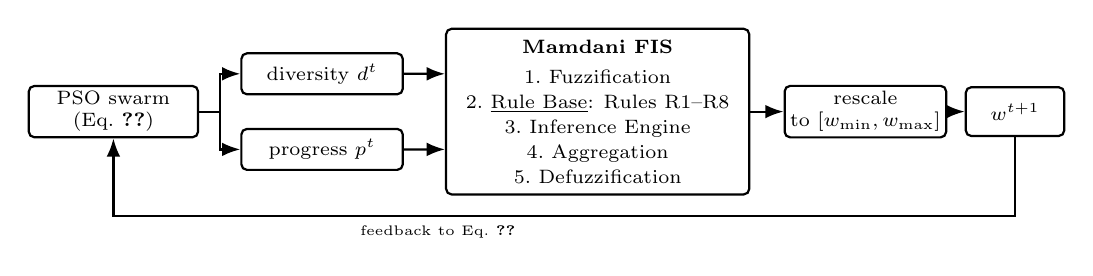
\begin{tikzpicture}[
    x=1cm,y=1cm,
    >=Latex,
    font=\scriptsize,
    block/.style={
        draw, thick, rounded corners=2pt,
        minimum height=0.62cm,
        minimum width=1.85cm,
        align=center,
        inner sep=2pt
    },
    inputblock/.style={
        draw, thick, rounded corners=2pt,
        minimum height=0.52cm,
        minimum width=2.05cm,
        align=center,
        inner sep=1.5pt
    },
    fis/.style={
        draw, thick, rounded corners=2pt,
        minimum height=2.0cm,
        minimum width=3.85cm,
        align=center,
        inner sep=4pt
    },
    sig/.style={->, thick},
    ann/.style={font=\tiny}
]

% --- Fixed coordinates to avoid overlaps after resizing ---
\node[block, minimum width=2.15cm] (pso) at (0,0)
{PSO swarm\\(Eq.~\ref{eq:velocity})};

\node[inputblock] (div) at (2.65,0.48)
{diversity $d^{t}$};

\node[inputblock] (prog) at (2.65,-0.48)
{progress $p^{t}$};

\node[fis] (fis) at (6.15,0)
{\textbf{Mamdani FIS}\\[3pt]
1.~Fuzzification\\[1pt]
2.~\underline{Rule Base}: Rules R1--R8\\[1pt]
3.~Inference Engine\\[1pt]
4.~Aggregation\\[1pt]
5.~Defuzzification};

\node[block, minimum width=2.0cm] (resc) at (9.55,0)
{rescale\\to $[w_{\min},w_{\max}]$};

\node[block, minimum width=1.25cm] (w) at (11.45,0)
{$w^{t+1}$};

% --- Input extraction from PSO ---
\coordinate (tap) at (1.35,0);

\draw[sig] (pso.east) -- (tap) |- (div.west);
\draw[sig] (tap) |- (prog.west);

% --- Inputs to FIS ---
\draw[sig] (div.east) -- ([yshift=0.48cm]fis.west);
\draw[sig] (prog.east) -- ([yshift=-0.48cm]fis.west);

% --- Main output path ---
\draw[sig] (fis.east) -- (resc.west);
\draw[sig] (resc.east) -- (w.west);

% --- Feedback path ---
\draw[sig] (w.south) -- ++(0,-1.00) -| (pso.south)
    node[pos=0.32, below, ann] {feedback to Eq.~\ref{eq:velocity}};

% --- Compact internal specification label ---
%\node[ann, anchor=north] at ($(fis.south)+(0,-0.05)$)
%{rules R1--R8};

\end{tikzpicture}%
}
\caption{PSO-FCS architecture.}
\label{fig:fcs}
\end{figure}

\textbf{Canonical PSO.} A swarm of $N$ particles searches the $D$-dimensional bounded box $[lb,\,ub]^{D}$ for $T$ iterations. Each particle $i \in \{1,\dots,N\}$ holds a position $\mathbf{x}_i^{t}\in\mathbb{R}^{D}$ and a velocity $\mathbf{v}_i^{t}\in\mathbb{R}^{D}$ at iteration $t$, together with its own best-so-far position $\mathbf{p}_i^{t}$ (\emph{pBest}). The swarm shares its global best-so-far position $\mathbf{g}^{t}$ (\emph{gBest}). At every iteration the particles update by the canonical equations~\cite{kennedy1995,shi1998}
\begin{equation}\label{eq:velocity}
\mathbf{v}_i^{t+1} = \underbrace{w\,\mathbf{v}_i^{t}}_{\text{inertia}} + \underbrace{c_1\,\mathbf{r}_1 \odot (\mathbf{p}_i^{t}-\mathbf{x}_i^{t})}_{\text{cognitive}} + \underbrace{c_2\,\mathbf{r}_2 \odot (\mathbf{g}^{t}-\mathbf{x}_i^{t})}_{\text{social}},
\quad \mathbf{x}_i^{t+1} = \mathbf{x}_i^{t} + \mathbf{v}_i^{t+1},
\end{equation}
where $w \in [w_{\min}, w_{\max}]$ is the inertia weight (the parameter studied in this paper), $c_1$ and $c_2$ are the cognitive and social acceleration coefficients, $\mathbf{r}_1,\mathbf{r}_2 \sim \mathcal{U}([0,1]^{D})$ are independent uniform random vectors drawn at every iteration, and $\odot$ denotes the element-wise (Hadamard) product. Velocities are clipped to $\pm V_{\max} = 0.1\,(ub-lb)$ to avoid divergence. The baseline PSO-STD uses the linear schedule $w(t) = w_{\max} - (w_{\max}-w_{\min})\,t/T$, decaying from $w_{\max}=0.9$ to $w_{\min}=0.1$ over $T$ iterations. The fuzzy variants (PSO-FCS) replace this schedule by the controller described below; everything else in Eq.~\eqref{eq:velocity} is identical.

\textbf{Mamdani controller.} A Mamdani FIS is the natural fit for this task: it represents the mapping from swarm state to $w$ as a small set of human-readable IF--THEN rules whose semantics can be edited, ablated and audited one rule at a time --- a property that opaque feedback laws or learned policies do not share, and that the present sensitivity study explicitly exploits. The controller maps two normalised state descriptors into $w$: the swarm diversity $d^{t} = D^{t}/D_{\max}^{t} \in [0,1]$ (with $D^{t}$ the mean swarm-to-centroid Euclidean distance and $D_{\max}^{t}$ its running maximum), and the iteration progress $p^{t} = t/T \in [0,1]$. The output $w$ is constrained to the same range $[w_{\min},w_{\max}] = [0.1, 0.9]$ as PSO-STD. Inference uses min--max operators (T-norm minimum for rule firing, S-norm maximum for output aggregation) on a discretised universe of $501$ points in $[0,1]$, followed by Centre-Of-Gravity (COG) defuzzification and a linear rescaling that maps the achievable centroid range $[c_{\min}, c_{\max}]$ of the output partition to $[w_{\min}, w_{\max}]$. The rescaling step compensates for the centroid compression at the boundaries, so that extreme rules can actually deliver $w \approx w_{\min}$ or $w_{\max}$.

\textbf{Membership functions and rule base.} A \emph{rule base} is the table that assigns one output linguistic term to every combination of input linguistic terms; it is the structural component varied in this study. To isolate it, the input and output partitions are held identical across all configurations. Input MFs ($d$ and $p$) are uniform triangulars: each label spans one label-width to either side of its centre with no shoulder at the boundaries. Output MFs ($w$) share the same uniform spacing but carry shoulder degeneracies at the two extreme labels, ensuring the full range $[w_{\min}, w_{\max}]$ is attainable after COG defuzzification. Table~\ref{tab:mf} lists the centres for inputs and output at each granularity. 
The rule base is therefore the \emph{only} component that varies across configurations.



\begin{table}[H]
\scriptsize
\centering
\caption{Triangular MF centres on $[0,1]$; inputs ($d$, $p$) have no shoulders, output ($w$) extreme labels carry shoulder degeneracies ($\dagger$).}\label{tab:mf}
\setlength{\tabcolsep}{4pt}
\begin{tabular}{lll ccccc}
\toprule
Gran. & Var. & Labels & \multicolumn{5}{c}{Centres on $[0,1]$} \\
\midrule
\multirow{2}{*}{3L} & input   & low / med / high    & 0.20 & 0.50 & 0.80 & ---  & ---  \\
                    & output$^\dagger$ & low / med / high    & 0.00 & 0.50 & 1.00 & ---  & ---  \\
\midrule
\multirow{2}{*}{5L} & input   & vl / l / m / h / vh & 0.15 & 0.35 & 0.50 & 0.65 & 0.85 \\
                    & output$^\dagger$ & vl / l / m / h / vh & 0.00 & 0.33 & 0.50 & 0.67 & 1.00 \\
\bottomrule
\multicolumn{8}{l}{\footnotesize $\dagger$\,Shoulder at boundary (membership 1 at $[0,1]$ endpoints).}
\end{tabular}
\end{table}



% ============================================================
\section{Experimental Design}\label{sec:experiments}
% ============================================================

\subsection{Rule Base Variants}\label{sec:rule_variants}

% Eight rule bases R1--R8 are generated by the additive factorial design described in Section~\ref{sec:rule_variants}, instantiated at $3 \times 3 = 9$ rules (3L) or $5 \times 5 = 25$ rules (5L) per base. Tables~\ref{tab:rules3L} and~\ref{tab:rules5L} report the resulting rule tables at three and five labels, respectively.

Eight rule bases R1--R8 are constructed by combining two independent semantic axes: a \emph{progress axis} that encodes how $w$ should evolve as iterations advance (decreasing $\downarrow$, increasing $\uparrow$, or neutral $-$), and a \emph{diversity axis} that encodes how $w$ should react to the current spread of the swarm (amplifying $\rightarrow$, compensating $\leftarrow$, or neutral $-$). R1 encodes the classical ``explore early, exploit late'' intuition by decreasing $w$ with progress and ignoring diversity; R2 is its deliberately counter-intuitive mirror. R3 and R4 test whether diversity reaction alone can substitute for progress guidance. R5--R8 combine each progress direction with each diversity reaction, forming the four sign combinations of the two non-neutral axes. The pairs (R1,\,R2), (R3,\,R4), (R5,\,R8) and (R6,\,R7) are orthogonal mirrors that invert exactly one factor, enabling clean attribution of any performance difference to a single semantic axis.

The rule tables are generated systematically: each cell $(p, d)$ is assigned the output label corresponding to $\mathrm{clip}(e_{\text{prog}}(p) + e_{\text{div}}(d))$, where $e_{\text{prog}}$ and $e_{\text{div}}$ are the integer encodings of the two axes and $\mathrm{clip}(\cdot)$ saturates the sum to the valid label range ($\{-1,0,+1\}$ at three labels, $\{-2,\dots,+2\}$ at five). This ensures every rule base is a deterministic function of two orthogonal design choices and can be reproduced exactly from Tables~\ref{tab:rules3L} and~\ref{tab:rules5L}; column headers E/M/L stand for early/mid/late (progress) and row labels L/M/H for low/med/high (diversity).

\begin{table}[H]
\scriptsize
\centering
\vspace{3pt}
\caption{Three-label rule bases R1--R8 (rows: diversity, columns: progress; L/M/H = low/med/high).}\label{tab:rules3L}
\setlength{\tabcolsep}{4pt}
\begin{tabular}{l|ccc|ccc|ccc|ccc}
\toprule
& \multicolumn{3}{c|}{R1 (P\,$\downarrow$, D\,---)}
& \multicolumn{3}{c|}{R2 (P\,$\uparrow$, D\,---)}
& \multicolumn{3}{c|}{R3 (P\,---, D\,$\rightarrow$)}
& \multicolumn{3}{c}{R4 (P\,---, D\,$\leftarrow$)} \\
Div\,$\backslash$\,Prog & E & M & L & E & M & L & E & M & L & E & M & L \\
\midrule
low    & H & M & L & L & M & H & L & L & L & H & H & H \\
medium & H & M & L & L & M & H & M & M & M & M & M & M \\
high   & H & M & L & L & M & H & H & H & H & L & L & L \\
\bottomrule
\toprule
& \multicolumn{3}{c|}{R5 (P\,$\downarrow$, D\,$\rightarrow$)}
& \multicolumn{3}{c|}{R6 (P\,$\downarrow$, D\,$\leftarrow$)}
& \multicolumn{3}{c|}{R7 (P\,$\uparrow$, D\,$\rightarrow$)}
& \multicolumn{3}{c}{R8 (P\,$\uparrow$, D\,$\leftarrow$)} \\
Div\,$\backslash$\,Prog & E & M & L & E & M & L & E & M & L & E & M & L \\
\midrule
low    & M & L & L & H & H & M & L & L & M & M & H & H \\
medium & H & M & L & H & M & L & L & M & H & L & M & H \\
high   & H & H & M & M & L & L & M & H & H & L & L & M \\
\bottomrule
\end{tabular}

\vspace{1pt}
\caption{Five-label rule bases R1--R8 (rows: diversity 1--5, columns: progress 1--5; \textbf{vl}/\textbf{l}/\textbf{m}/\textbf{h}/\textbf{vh} = very\_low/low/med/high/very\_high).}\label{tab:rules5L}
\setlength{\tabcolsep}{2pt}
\begin{tabular}{l|ccccc|ccccc|ccccc|ccccc}
\toprule
& \multicolumn{5}{c|}{R1 (P\,$\downarrow$, D\,---)}
& \multicolumn{5}{c|}{R2 (P\,$\uparrow$, D\,---)}
& \multicolumn{5}{c|}{R3 (P\,---, D\,$\rightarrow$)}
& \multicolumn{5}{c}{R4 (P\,---, D\,$\leftarrow$)} \\
D\,$\backslash$\,P & 1 & 2 & 3 & 4 & 5 & 1 & 2 & 3 & 4 & 5 & 1 & 2 & 3 & 4 & 5 & 1 & 2 & 3 & 4 & 5 \\
\midrule
1 & vh & h  & m  & l  & vl & vl & l  & m  & h  & vh & vl & vl & vl & vl & vl & vh & vh & vh & vh & vh \\
2 & vh & h  & m  & l  & vl & vl & l  & m  & h  & vh & l  & l  & l  & l  & l  & h  & h  & h  & h  & h  \\
3 & vh & h  & m  & l  & vl & vl & l  & m  & h  & vh & m  & m  & m  & m  & m  & m  & m  & m  & m  & m  \\
4 & vh & h  & m  & l  & vl & vl & l  & m  & h  & vh & h  & h  & h  & h  & h  & l  & l  & l  & l  & l  \\
5 & vh & h  & m  & l  & vl & vl & l  & m  & h  & vh & vh & vh & vh & vh & vh & vl & vl & vl & vl & vl \\
\bottomrule
\toprule
& \multicolumn{5}{c|}{R5 (P\,$\downarrow$, D\,$\rightarrow$)}
& \multicolumn{5}{c|}{R6 (P\,$\downarrow$, D\,$\leftarrow$)}
& \multicolumn{5}{c|}{R7 (P\,$\uparrow$, D\,$\rightarrow$)}
& \multicolumn{5}{c}{R8 (P\,$\uparrow$, D\,$\leftarrow$)} \\
D\,$\backslash$\,P & 1 & 2 & 3 & 4 & 5 & 1 & 2 & 3 & 4 & 5 & 1 & 2 & 3 & 4 & 5 & 1 & 2 & 3 & 4 & 5 \\
\midrule
1 & m  & l  & vl & vl & vl & vh & vh & vh & h  & m  & vl & vl & vl & l  & m  & m  & h  & vh & vh & vh \\
2 & h  & m  & l  & vl & vl & vh & vh & h  & m  & l  & vl & vl & l  & m  & h  & l  & m  & h  & vh & vh \\
3 & vh & h  & m  & l  & vl & vh & h  & m  & l  & vl & vl & l  & m  & h  & vh & vl & l  & m  & h  & vh \\
4 & vh & vh & h  & m  & l  & h  & m  & l  & vl & vl & l  & m  & h  & vh & vh & vl & vl & l  & m  & h  \\
5 & vh & vh & vh & h  & m  & m  & l  & vl & vl & vl & m  & h  & vh & vh & vh & vl & vl & vl & l  & m  \\
\bottomrule
\end{tabular}
\end{table}

% Explanatory diagram for clip(.) intentionally kept commented out: the
% textual explanation above (with explicit support sets) was deemed
% sufficient. Re-enable the figure if a visual aid becomes necessary.
% % diagram_clip.tex
% Visual explanation of the clip(.) operator used in the additive rule design
% (Eq. \ref{eq:additive_rule}). Designed to be \input{} from paper_wea2026.tex.
%
% Requires: \usepackage{tikz}
%
% Idea: e_prog and e_div are integer effects on a discrete label axis.
% Their sum may fall outside the available label range; clip(.) snaps it back
% to the nearest extreme label so that the additive design always yields a
% valid output linguistic term.
%
% Example shown: 3-label case, support {-1, 0, +1} mapped to {L, M, H}.
% e_prog = +1 (toward H), e_div = +1 (toward H), sum = +2 -> clipped to +1 = H.
%
\begin{figure}[h]
\centering
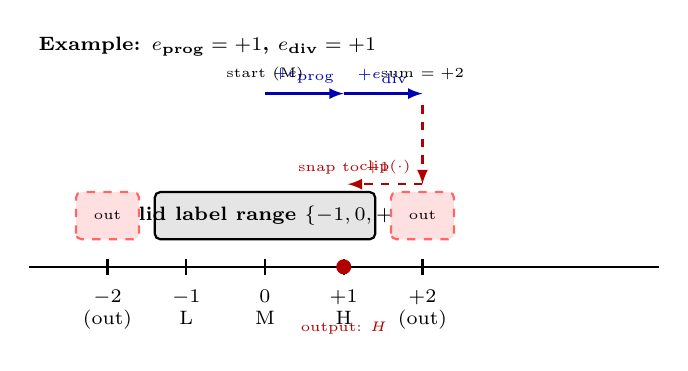
\begin{tikzpicture}[
    >=latex, font=\scriptsize,
    label/.style={font=\scriptsize\bfseries},
    tick/.style={thick},
    eff/.style={->, thick},
    clipline/.style={->, thick, dashed},
    valid/.style={fill=black!10, draw=black, thick, rounded corners=2pt},
    outside/.style={fill=red!12, draw=red!60, thick, dashed, rounded corners=2pt}
]
% ---- label axis (3L) ----
\draw[tick] (-3,0) -- (5,0);
\foreach \x/\lab in {-2/{$-2$\\(out)}, -1/{$-1$\\L}, 0/{$0$\\M}, 1/{$+1$\\H}, 2/{$+2$\\(out)}} {
    \draw[tick] (\x,0.1) -- (\x,-0.1);
    \node[align=center, below=2pt] at (\x,-0.1) {\lab};
}
% valid region
\draw[valid] (-1.4,0.35) rectangle (1.4,0.95);
\node[label] at (0,0.65) {valid label range $\{-1,0,+1\}$};

% out-of-range region (left)
\draw[outside] (-2.4,0.35) rectangle (-1.6,0.95);
\node[font=\tiny] at (-2,0.65) {out};
% out-of-range region (right)
\draw[outside] (1.6,0.35) rectangle (2.4,0.95);
\node[font=\tiny] at (2,0.65) {out};

% additive composition arrows above
\node[label, anchor=west] at (-3.0,2.8) {Example: $e_{\text{prog}}=+1$, $e_{\text{div}}=+1$};
\draw[eff, blue!70!black] (0,2.2) -- (1,2.2)
    node[midway, above, font=\tiny] {$+e_{\text{prog}}$};
\draw[eff, blue!70!black] (1,2.2) -- (2,2.2)
    node[midway, above, font=\tiny] {$+e_{\text{div}}$};
\node[font=\tiny] at (0,2.45) {start (M)};
\node[font=\tiny] at (2.0,2.45) {sum $=+2$};

% drop down to axis
\draw[clipline, red!70!black] (2,2.05) -- (2,1.05);
% clip arrow snapping back to +1
\draw[clipline, red!70!black] (2,1.05) -- (1.05,1.05)
    node[midway, above, font=\tiny] {$\mathrm{clip}(\cdot)$};
\node[font=\tiny, red!70!black] at (1,1.25) {snap to $+1$};

% final dot
\filldraw[red!70!black] (1,0) circle (2.5pt);
\node[font=\tiny, red!70!black, below=12pt] at (1,-0.15) {output: $H$};

\end{tikzpicture}
\caption{Geometric meaning of $\mathrm{clip}(\cdot)$ in Eq.~\eqref{eq:additive_rule}. The two semantic effects $e_{\text{prog}}$ and $e_{\text{div}}$ are added on the integer label axis. If their sum lies inside the valid label range it is used directly; if it falls outside (here $+2$ at three labels), $\mathrm{clip}(\cdot)$ snaps it to the nearest extreme label ($H$). The same convention applies symmetrically on the negative side and at five labels with support $\{-2,\dots,+2\}$.}
\label{fig:clip}
\end{figure}


\subsection{Benchmarks, Configuration and Statistical Methodology}

\textbf{Benchmark suite.} We use a six-function subset of the classical F1--F23 benchmark set~\cite{abualigah2021aoa} spanning three difficulty categories: F1 Sphere (unimodal, $D=100$), F5 Rosenbrock (narrow-valley, $D=100$), and F11 Griewank (multimodal scalable, $D=100$), and the fixed-dimension Shekel family F21--F23 with $5$, $7$ and $10$ components respectively ($D=4$, with non-zero optima $-10.153$, $-10.403$, $-10.536$). To avoid scale-mixing artefacts, statistical tests are reported both on the full set and disaggregated by \textit{optimum group}: \textit{optimum~$=0$} (F1, F5, F11) and \textit{optimum~$\neq 0$} (F21--F23).

\textbf{PSO configuration.} All seventeen configurations share the same PSO core: $N=20$ particles, $T=1{,}000$ iterations, $c_1=c_2=2.0$, velocity clipping at $\pm 0.1\,(ub-lb)$, $31$ independent runs with reproducible seed. The fuzzy variants use the triangular partition defined in Table~\ref{tab:mf}, Mamdani min--max inference, COG defuzzification with rescaling, and effective range $w \in [0.1, 0.9]$. The baseline PSO-STD uses the linear schedule $w(t) = 0.9 - 0.8\,t/T$ (decay from $0.9$ to $0.1$)~\cite{shi1998}. In total: $17 \times 6 \times 31 = 3{,}162$ runs.

\textbf{Statistical methodology.} Pairwise comparisons use the Wilcoxon signed-rank test~\cite{wilcoxon1945} with Holm--Bonferroni correction~\cite{holm1979} ($\alpha=0.05$); effect sizes use Cohen's~$d$ with the conventional small/medium/large thresholds~\cite{cohen1988}. A global ranking is built with the Friedman test~\cite{friedman1937} on mean fitness, repeated by optimum group. Mirror pairs are compared with Mann--Whitney $U$. Full numerical output is available from the authors on request.

% ============================================================
\section{Results and Discussion}\label{sec:results}
% ============================================================

% The seventeen configurations were executed under identical conditions, producing $3{,}162$ independent runs. We report the analysis at three increasing levels of disaggregation: (i) a global ranking across all six functions; (ii) a stratified analysis by optimum group; and (iii) targeted comparisons isolating individual factors of the orthogonal design (mirror pairs, granularity, factorial interaction, and inertia weight trajectories).

\subsection{Overall Ranking Across All Functions}\label{sec:results_global}

The Friedman test on the matrix of mean fitness values rejects the null hypothesis of equal performance with $\chi^2 = 49.46$ ($p = 2.79\times 10^{-5}$), confirming that rule base structure does have a measurable effect on PSO performance. Table~\ref{tab:rankings} reports the global ranking (a) and its per-function disaggregation (b). The global order exhibits a clear monotone structure: the top six positions are occupied exclusively by configurations whose progress effect is decreasing (R1, R5, R6 and PSO-STD), while the bottom five are dominated by progress-increasing variants. R1 wins at both granularities; R1-5L outperforms PSO-STD by $2.7$ rank units. Per function, PSO-STD, R1-5L and R5-5L dominate the optimum-zero columns (F1, F5, F11), whereas the Shekel columns (F21--F23) reorder configurations almost arbitrarily, foreshadowing Section~\ref{sec:results_optgroup}.

\begin{table}[H]
\scriptsize
\centering
\caption{Friedman rankings ($\chi^2\!=\!49.46$, $p\!=\!2.79\!\times\!10^{-5}$, lower is better): (a)~global mean ranks; (b)~per-function disaggregation, row $k$ = config.~ranked $k$-th on $F_i$.}\label{tab:rankings}\label{tab:friedman_global}\label{tab:per_function_ranking}
\setlength{\tabcolsep}{2pt}
\resizebox{\textwidth}{!}{%
\begin{tabular}{rlc @{\hspace{10pt}} |c|cccccc}
\toprule
\multicolumn{3}{c}{\textbf{(a) Global ranking}} & \multicolumn{7}{c}{\textbf{(b) Per-function ranking}} \\
\cmidrule(r){1-3}\cmidrule(l){4-10}
\# & Config & Rank & Pos. & F1 & F5 & F11 & F21 & F22 & F23 \\
\midrule
1  & \textbf{R1-5L} & 2.83  & 1  & \textbf{PSO-STD} & \textbf{PSO-STD} & \textbf{PSO-STD} & \textbf{R7-3L}   & \textbf{R6-3L}   & \textbf{R1-3L} \\
2  & R1-3L          & 4.00  & 2  & R1-5L            & R1-5L            & R1-5L            & R5-3L            & R4-3L            & R1-5L          \\
3  & R5-3L          & 5.17  & 3  & R5-5L            & R5-5L            & R1-3L            & R5-5L            & R1-5L            & R4-5L          \\
4  & PSO-STD        & 5.50  & 4  & R1-3L            & R1-3L            & R5-5L            & R6-3L            & R1-3L            & R5-3L          \\
5  & R6-3L          & 6.67  & 5  & R5-3L            & R5-3L            & R5-3L            & R4-5L            & R3-3L            & R4-3L          \\
6  & R5-5L          & 7.17  & 6  & R6-3L            & R6-5L            & R6-5L            & R1-5L            & R6-5L            & R3-3L          \\
7  & R4-3L          & 7.33  & 7  & R6-5L            & R6-3L            & R6-3L            & R4-3L            & R8-3L            & PSO-STD        \\
8  & R4-5L          & 8.17  & 8  & R8-3L            & R8-3L            & R8-3L            & R1-3L            & R4-5L            & R8-3L          \\
9  & R8-3L          & 8.67  & 9  & R8-5L            & R8-5L            & R8-5L            & R2-5L            & PSO-STD          & R3-5L          \\
10 & R6-5L          & 8.83  & 10 & R4-3L            & R4-3L            & R4-3L            & R3-3L            & R5-3L            & R7-5L          \\
11 & R3-3L          & 10.17 & 11 & R4-5L            & R4-5L            & R4-5L            & R2-3L            & R2-3L            & R2-3L          \\
12 & R7-3L          & 12.00 & 12 & R2-3L            & R3-5L            & R2-3L            & R6-5L            & R7-3L            & R2-5L          \\
13 & R2-3L          & 12.00 & 13 & R3-3L            & R7-3L            & R3-3L            & R8-3L            & R7-5L            & R5-5L          \\
14 & R8-5L          & 12.33 & 14 & R3-5L            & R3-3L            & R7-3L            & PSO-STD          & R2-5L            & R8-5L          \\
15 & R3-5L          & 13.50 & 15 & R7-3L            & R2-3L            & R3-5L            & R7-5L            & R3-5L            & R6-3L          \\
16 & R2-5L          & 14.00 & 16 & R2-5L            & R2-5L            & R7-5L            & R3-5L            & R8-5L            & R6-5L          \\
17 & R7-5L          & 14.67 & 17 & R7-5L            & R7-5L            & R2-5L            & R8-5L            & R5-5L            & R7-3L          \\
\bottomrule
\end{tabular}}
\end{table}


% % \vspace{-0.50cm}
% \begin{table}[H]
% \scriptsize
% \caption{Global Friedman ranking ($\chi^2=49.46$, $p=2.79\!\times\!10^{-5}$); lower is better.}\label{tab:friedman_global}
% \centering
% \begin{tabular}{rlc rlc rlc}
% \toprule
% \# & Config & Rank & \# & Config & Rank & \# & Config & Rank \\
% \midrule
% 1 & \textbf{R1-5L}  & 2.83 & 7  & R4-3L  & 7.33  & 13 & R2-3L  & 12.00 \\
% 2 & R1-3L           & 4.00 & 8  & R4-5L  & 8.17  & 14 & R8-5L  & 12.33 \\
% 3 & R5-3L           & 5.17 & 9  & R8-3L  & 8.67  & 15 & R3-5L  & 13.50 \\
% 4 & PSO-STD         & 5.50 & 10 & R6-5L  & 8.83  & 16 & R2-5L  & 14.00 \\
% 5 & R6-3L           & 6.67 & 11 & R3-3L  & 10.17 & 17 & R7-5L  & 14.67 \\
% 6 & R5-5L           & 7.17 & 12 & R7-3L  & 12.00 &    &        &       \\
% \bottomrule
% \end{tabular}
% \end{table}





% \begin{table}[H]
% \scriptsize
% \caption{Per-function ranking by mean fitness; row $k$ in column $F_i$ = configuration ranked $k$-th on $F_i$.}\label{tab:per_function_ranking}
% \centering
% % \setlength{\tabcolsep}{4pt}
% \scriptsize
% \begin{tabular}{c|cccccc}
% \toprule
% Pos. & F1 & F5 & F11 & F21 & F22 & F23 \\
% \midrule
% 1  & \textbf{PSO-STD} & \textbf{PSO-STD} & \textbf{PSO-STD} & \textbf{R7-3L}   & \textbf{R6-3L}   & \textbf{R1-3L} \\
% 2  & R1-5L            & R1-5L            & R1-5L            & R5-3L            & R4-3L            & R1-5L          \\
% 3  & R5-5L            & R5-5L            & R1-3L            & R5-5L            & R1-5L            & R4-5L          \\
% 4  & R1-3L            & R1-3L            & R5-5L            & R6-3L            & R1-3L            & R5-3L          \\
% 5  & R5-3L            & R5-3L            & R5-3L            & R4-5L            & R3-3L            & R4-3L          \\
% 6  & R6-3L            & R6-5L            & R6-5L            & R1-5L            & R6-5L            & R3-3L          \\
% 7  & R6-5L            & R6-3L            & R6-3L            & R4-3L            & R8-3L            & PSO-STD        \\
% 8  & R8-3L            & R8-3L            & R8-3L            & R1-3L            & R4-5L            & R8-3L          \\
% 9  & R8-5L            & R8-5L            & R8-5L            & R2-5L            & PSO-STD          & R3-5L          \\
% 10 & R4-3L            & R4-3L            & R4-3L            & R3-3L            & R5-3L            & R7-5L          \\
% 11 & R4-5L            & R4-5L            & R4-5L            & R2-3L            & R2-3L            & R2-3L          \\
% 12 & R2-3L            & R3-5L            & R2-3L            & R6-5L            & R7-3L            & R2-5L          \\
% 13 & R3-3L            & R7-3L            & R3-3L            & R8-3L            & R7-5L            & R5-5L          \\
% 14 & R3-5L            & R3-3L            & R7-3L            & PSO-STD          & R2-5L            & R8-5L          \\
% 15 & R7-3L            & R2-3L            & R3-5L            & R7-5L            & R3-5L            & R6-3L          \\
% 16 & R2-5L            & R2-5L            & R7-5L            & R3-5L            & R8-5L            & R6-5L          \\
% 17 & R7-5L            & R7-5L            & R2-5L            & R8-5L            & R5-5L            & R7-3L          \\
% \bottomrule
% \end{tabular}
% \end{table}


 





\subsection{Performance by Optimum Group}\label{sec:results_optgroup}

Aggregating heterogeneous fitness scales can mask category-specific behaviour. We therefore repeat the Friedman analysis on each optimum group (Table~\ref{tab:friedman_byopt}). On the optimum-zero group (F1,\,F5,\,F11) the test rejects the null hypothesis with $p = 6.07\times 10^{-5}$: PSO-STD takes the first place, followed closely by R1-5L, R5-5L and R1-3L, while progress-increasing variants R2 and R7 fall to the bottom. On the optimum-non-zero group (F21--F23) the Friedman test does \emph{not} reject the null hypothesis ($p = 0.088$), and the ordering becomes essentially flat: the best fuzzy configuration R1-5L achieves a mean rank of $3.67$, while PSO-STD itself drops to position~9. With only three functions per group, these rankings should be interpreted as indicative rather than conclusive. This stratification confirms that rule base structure has a noticeable impact on the high-dimensional optimum-zero functions and a much weaker, statistically inconclusive impact on the four-dimensional Shekel functions, where the deceptive multi-foxhole landscape appears to dominate over the inertia weight schedule.


% \begin{table}[H]
% \scriptsize
% \caption{Friedman ranking by optimum group (top~6 and bottom~3 shown); lower is better.}\label{tab:friedman_byopt}
% \centering
% \setlength{\tabcolsep}{4pt}
% \begin{tabular}{rlc | rlc}
% \toprule
% \multicolumn{3}{c|}{\textbf{Optimum $=0$} \quad ($\chi^2=47.32,\,p=6.07\!\times\!10^{-5}$)}
% & \multicolumn{3}{c}{\textbf{Optimum $\neq 0$} \quad ($\chi^2=24.08,\,p=0.088$)} \\
% \# & Config & Rank & \# & Config & Rank \\
% \midrule
% 1  & \textbf{PSO-STD} & 1.00  & 1  & \textbf{R1-5L} & 3.67  \\
% 2  & R1-5L            & 2.00  & 2  & R1-3L          & 4.33  \\
% 3  & R5-5L            & 3.33  & 3  & R4-3L          & 4.67  \\
% 4  & R1-3L            & 3.67  & 4  & R5-3L          & 5.33  \\
% 5  & R5-3L            & 5.00  & 5  & R4-5L          & 5.33  \\
% 6  & R6-5L            & 6.33  & 6  & R6-3L          & 6.67  \\
% \multicolumn{3}{c|}{\vdots} & \multicolumn{3}{c}{\vdots} \\
% 15 & R7-3L            & 14.00 & 15 & R7-5L          & 12.67 \\
% 16 & R2-5L            & 16.33 & 16 & R3-5L          & 13.33 \\
% 17 & R7-5L            & 16.67 & 17 & R8-5L          & 15.67 \\
% \bottomrule
% \end{tabular}
% \end{table}
% 
\begin{table}[H]
\scriptsize
\caption{Friedman ranking by optimum group (all 17 configurations); lower is better.}\label{tab:friedman_byopt}
\centering
\setlength{\tabcolsep}{4pt}
\begin{tabular}{rlc | rlc}
\toprule
\multicolumn{3}{c|}{\textbf{Optimum $=0$} \quad ($\chi^2=47.32,\,p=6.07\!\times\!10^{-5}$)}
& \multicolumn{3}{c}{\textbf{Optimum $\neq 0$} \quad ($\chi^2=24.08,\,p=0.088$)} \\
\# & Config & Rank & \# & Config & Rank \\
\midrule
1  & \textbf{PSO-STD} & 1.00  & 1  & \textbf{R1-5L} & 3.67  \\
2  & R1-5L            & 2.00  & 2  & R1-3L          & 4.33  \\
3  & R5-5L            & 3.33  & 3  & R4-3L          & 4.67  \\
4  & R1-3L            & 3.67  & 4  & R5-3L          & 5.33  \\
5  & R5-3L            & 5.00  & 5  & R4-5L          & 5.33  \\
6  & R6-5L            & 6.33  & 6  & R6-3L          & 6.67  \\
7  & R6-3L            & 6.67  & 7  & R3-3L          & 7.00  \\
8  & R8-3L            & 8.00  & 8  & R8-3L          & 9.33  \\
9  & R8-5L            & 9.00  & 9  & PSO-STD        & 10.00 \\
10 & R4-3L            & 10.00 & 10 & R7-3L          & 10.00 \\
11 & R4-5L            & 11.00 & 11 & R2-3L          & 11.00 \\
12 & R2-3L            & 13.00 & 12 & R5-5L          & 11.00 \\
13 & R3-3L            & 13.33 & 13 & R6-5L          & 11.33 \\
14 & R3-5L            & 13.67 & 14 & R2-5L          & 11.67 \\
15 & R7-3L            & 14.00 & 15 & R7-5L          & 12.67 \\
16 & R2-5L            & 16.33 & 16 & R3-5L          & 13.33 \\
17 & R7-5L            & 16.67 & 17 & R8-5L          & 15.67 \\
\bottomrule
\end{tabular}
\end{table}
\subsection{Mirror-Pair Analysis: Isolating Individual Axes}\label{sec:mirror}

The orthogonal mirror pairs isolate the contribution of each semantic axis. Table~\ref{tab:mirror} summarises the Mann--Whitney $U$ tests on all four mirror pairs (3L). The progress-axis pair R1\,$\leftrightarrow$\,R2 yields the largest effect sizes in the dataset: on F1, F5 and F11 R1 dominates R2 with $|d|>3.5$ and $p<1.5\times 10^{-11}$; on F21--F23 the same pair yields $p>0.05$ and negligible $d$. A symmetric pattern is observed for the diversity-axis pair R3\,$\leftrightarrow$\,R4, where R4 (compensating) dominates R3 (following) on the optimum-zero functions with $|d|>3$. The combined-axis pair R6\,$\leftrightarrow$\,R7 replicates this split pattern ($|d|>3.5$, $p<10^{-11}$ on F1--F11; $p>0.05$ on F21--F23), confirming that progress direction dominates regardless of diversity polarity.




% \vspace{-0.50cm}

\begin{table}[H]
\scriptsize
\caption{Mirror-pair Mann--Whitney $U$ tests (3L). Effect size $d$ is signed relative to the first label of the pair.}\label{tab:mirror}
\centering
\setlength{\tabcolsep}{3pt}
\begin{tabular}{ll cc cc cc}
\toprule
& & \multicolumn{2}{c}{F1} & \multicolumn{2}{c}{F5} & \multicolumn{2}{c}{F11} \\
Pair & Winner & $d$ & $p$ & $d$ & $p$ & $d$ & $p$ \\
\midrule
R1\,$\leftrightarrow$\,R2 & R1 & $-8.03$ & $\,\,1.4\!\times\!10^{-11}$ & $-4.61$ & $\,\,1.4\!\times\!10^{-11}$ & $-7.11$ & $\,\,1.4\!\times\!10^{-11}$ \\
R3\,$\leftrightarrow$\,R4 & R4 & $\phantom{-}5.86$ & $\,\,1.4\!\times\!10^{-11}$ & $\phantom{-}3.77$ & $\,\,1.4\!\times\!10^{-11}$ & $\phantom{-}6.30$ & $\,\,1.4\!\times\!10^{-11}$ \\
R5\,$\leftrightarrow$\,R8 & R5 & $-3.50$ & $\,\,2.3\!\times\!10^{-11}$ & $-3.91$ & $\,\,1.9\!\times\!10^{-11}$ & $-3.41$ & $\,\,1.4\!\times\!10^{-11}$ \\
R6\,$\leftrightarrow$\,R7 & R6 & $-7.23$ & $\,\,1.4\!\times\!10^{-11}$ & $-3.59$ & $\,\,1.4\!\times\!10^{-11}$ & $-6.52$ & $\,\,1.4\!\times\!10^{-11}$ \\
\midrule
& & \multicolumn{2}{c}{F21} & \multicolumn{2}{c}{F22} & \multicolumn{2}{c}{F23} \\
& Winner & $d$ & $p$ & $d$ & $p$ & $d$ & $p$ \\
\midrule
R1\,$\leftrightarrow$\,R2 & R1 & $-0.04$ & $0.541$ & $-0.21$ & $0.767$ & $-0.41$ & $0.526$ \\
R3\,$\leftrightarrow$\,R4 & R4 & $\phantom{-}0.05$ & $0.247$ & $\phantom{-}0.11$ & $0.075$ & $\phantom{-}0.06$ & $0.265$ \\
R5\,$\leftrightarrow$\,R8 & R5 & $-0.28$ & $0.059$ & $\phantom{-}0.06$ & $0.539$ & $-0.10$ & $0.191$ \\
R6\,$\leftrightarrow$\,R7 & R6 & $\phantom{-}0.16$ & $0.112$ & $-0.38$ & $0.182$ & $-0.16$ & $0.434$ \\
\bottomrule
\end{tabular}
\end{table}



\subsection{Granularity Effect: 3 vs.\ 5 Labels}\label{sec:granularity}

Table~\ref{tab:granularity} compares each rule strategy at the two granularities. Three patterns emerge: (i)~for the best rule (R1), the 3L\,$\to$\,5L move improves F1 ($p=0.0045$, $d=0.78$) and is statistically equivalent elsewhere, so finer granularity \emph{refines} the dominant strategy; (ii)~for the diversity-compensating rule (R4) the change has the opposite sign with very large effect sizes ($|d|>2.3$, $p<10^{-9}$ on F1, F5, F11) --- when diversity is the only signal driving $w$, the smoother 5-label surface admits a wider range of high $w$ values that interfere with convergence in $100$ dimensions; (iii)~for the high-stagnation rule families (R3, R7) granularity is statistically inert across all six functions, and for R2 the only significant difference is a moderate degradation on F11 ($d=-0.69$, $p=0.008$).

\begin{table}[b]
\scriptsize
\caption{Granularity comparison (3L vs.\,5L) per rule, Mann--Whitney $U$ at $\alpha=0.05$; ``Winner'' = lower mean fitness (statistically significant or notable cases; 9 of 48 pairs).}\label{tab:granularity}
\centering
\begin{tabular}{ll rr cc}
\toprule
Rule & Function & Mean 3L & Mean 5L & Winner & Effect ($d$) \\
\midrule
R1 & F1  & $47.66$       & $33.26$       & 5L\textsuperscript{*}  & $\phantom{-}0.78$ \\
R1 & F5  & $1{,}534.39$  & $1{,}349.87$  & 5L                     & $\phantom{-}0.34$ \\
R4 & F1  & $1{,}756.69$  & $2{,}300.68$  & 3L\textsuperscript{*}  & $-3.16$ \\
R4 & F5  & $104{,}964.59$& $169{,}138.80$& 3L\textsuperscript{*}  & $-2.34$ \\
R4 & F11 & $16.59$       & $21.67$       & 3L\textsuperscript{*}  & $-3.17$ \\
R5 & F1  & $58.09$       & $47.65$       & 5L\textsuperscript{*}  & $\phantom{-}0.25$ \\
R5 & F5  & $2{,}151.32$  & $1{,}462.09$  & 5L\textsuperscript{*}  & $\phantom{-}0.62$ \\
R6 & F5  & $3{,}911.19$  & $3{,}041.92$  & 5L\textsuperscript{*}  & $\phantom{-}0.70$ \\
R2 & F11 & $103.22$      & $116.80$      & 3L\textsuperscript{*}  & $-0.69$ \\
\bottomrule
\multicolumn{6}{l}{\footnotesize \textsuperscript{*}\,Statistically significant at $\alpha=0.05$.}
\end{tabular}
\end{table}



\subsection{Factorial Interaction and Inertia Weight Behaviour}\label{sec:factorial}

The factorial layout in Table~\ref{tab:factorial} reports the mean fitness on the optimum-zero group for every combination of progress and diversity effects, at both granularities. Two patterns indicate a progress\,$\times$\,diversity interaction. First, the row Prog\,$\downarrow$ stays at $\sim 5\times 10^2$--$1.3\times 10^3$ across all three diversity levels, whereas the row Prog\,$\uparrow$ jumps to $\sim 10^6$ for both Div\,$\rightarrow$ and Div\,$-$ but collapses to $\sim 3\times 10^3$ when paired with Div\,$\leftarrow$ (R8). Second, in the row Prog\,$-$ the diversity-compensating effect (R4) reduces fitness by about an order of magnitude relative to the diversity-following or neutral cases (R3, no~rule); the same gap shrinks to a factor of $\sim 2$ in the Prog\,$\downarrow$ row (R6 vs.~R1) and is absent on the Shekel group (not shown, where all entries lie approximately in $[-7, -5]$). The benefit of compensating diversity is therefore conditional on a non-decreasing progress effect.

\vspace{-0.5cm}

\begin{table}[H]
\scriptsize
\caption{Factorial layout on the optimum-zero group: mean fitness over F1, F5, F11 at 3L\,/\,5L. The (Prog\,$-$, Div\,$-$) cell is empty by design (constant $w$).}\label{tab:factorial}
\centering
\setlength{\tabcolsep}{6pt}
\renewcommand{\arraystretch}{1.15}
\begin{tabular}{l|ccc}
\toprule
 & \textbf{Div\,$\rightarrow$} & \textbf{Div\,$-$} & \textbf{Div\,$\leftarrow$} \\
\midrule
\textbf{Prog\,$\downarrow$} & R5: $7.4\!\times\!10^{2}$ / $5.0\!\times\!10^{2}$ & R1: $5.3\!\times\!10^{2}$ / $4.6\!\times\!10^{2}$ & R6: $1.3\!\times\!10^{3}$ / $1.1\!\times\!10^{3}$ \\
\textbf{Prog\,$-$}          & R3: $1.1\!\times\!10^{6}$ / $9.6\!\times\!10^{5}$ & ---                                              & R4: $3.6\!\times\!10^{4}$ / $5.7\!\times\!10^{4}$ \\
\textbf{Prog\,$\uparrow$}   & R7: $1.0\!\times\!10^{6}$ / $1.3\!\times\!10^{6}$ & R2: $1.1\!\times\!10^{6}$ / $1.2\!\times\!10^{6}$ & R8: $3.0\!\times\!10^{3}$ / $3.6\!\times\!10^{3}$ \\
\bottomrule
\end{tabular}
\end{table}

\vspace{-0.5cm}

\begin{figure}[H]
\centering
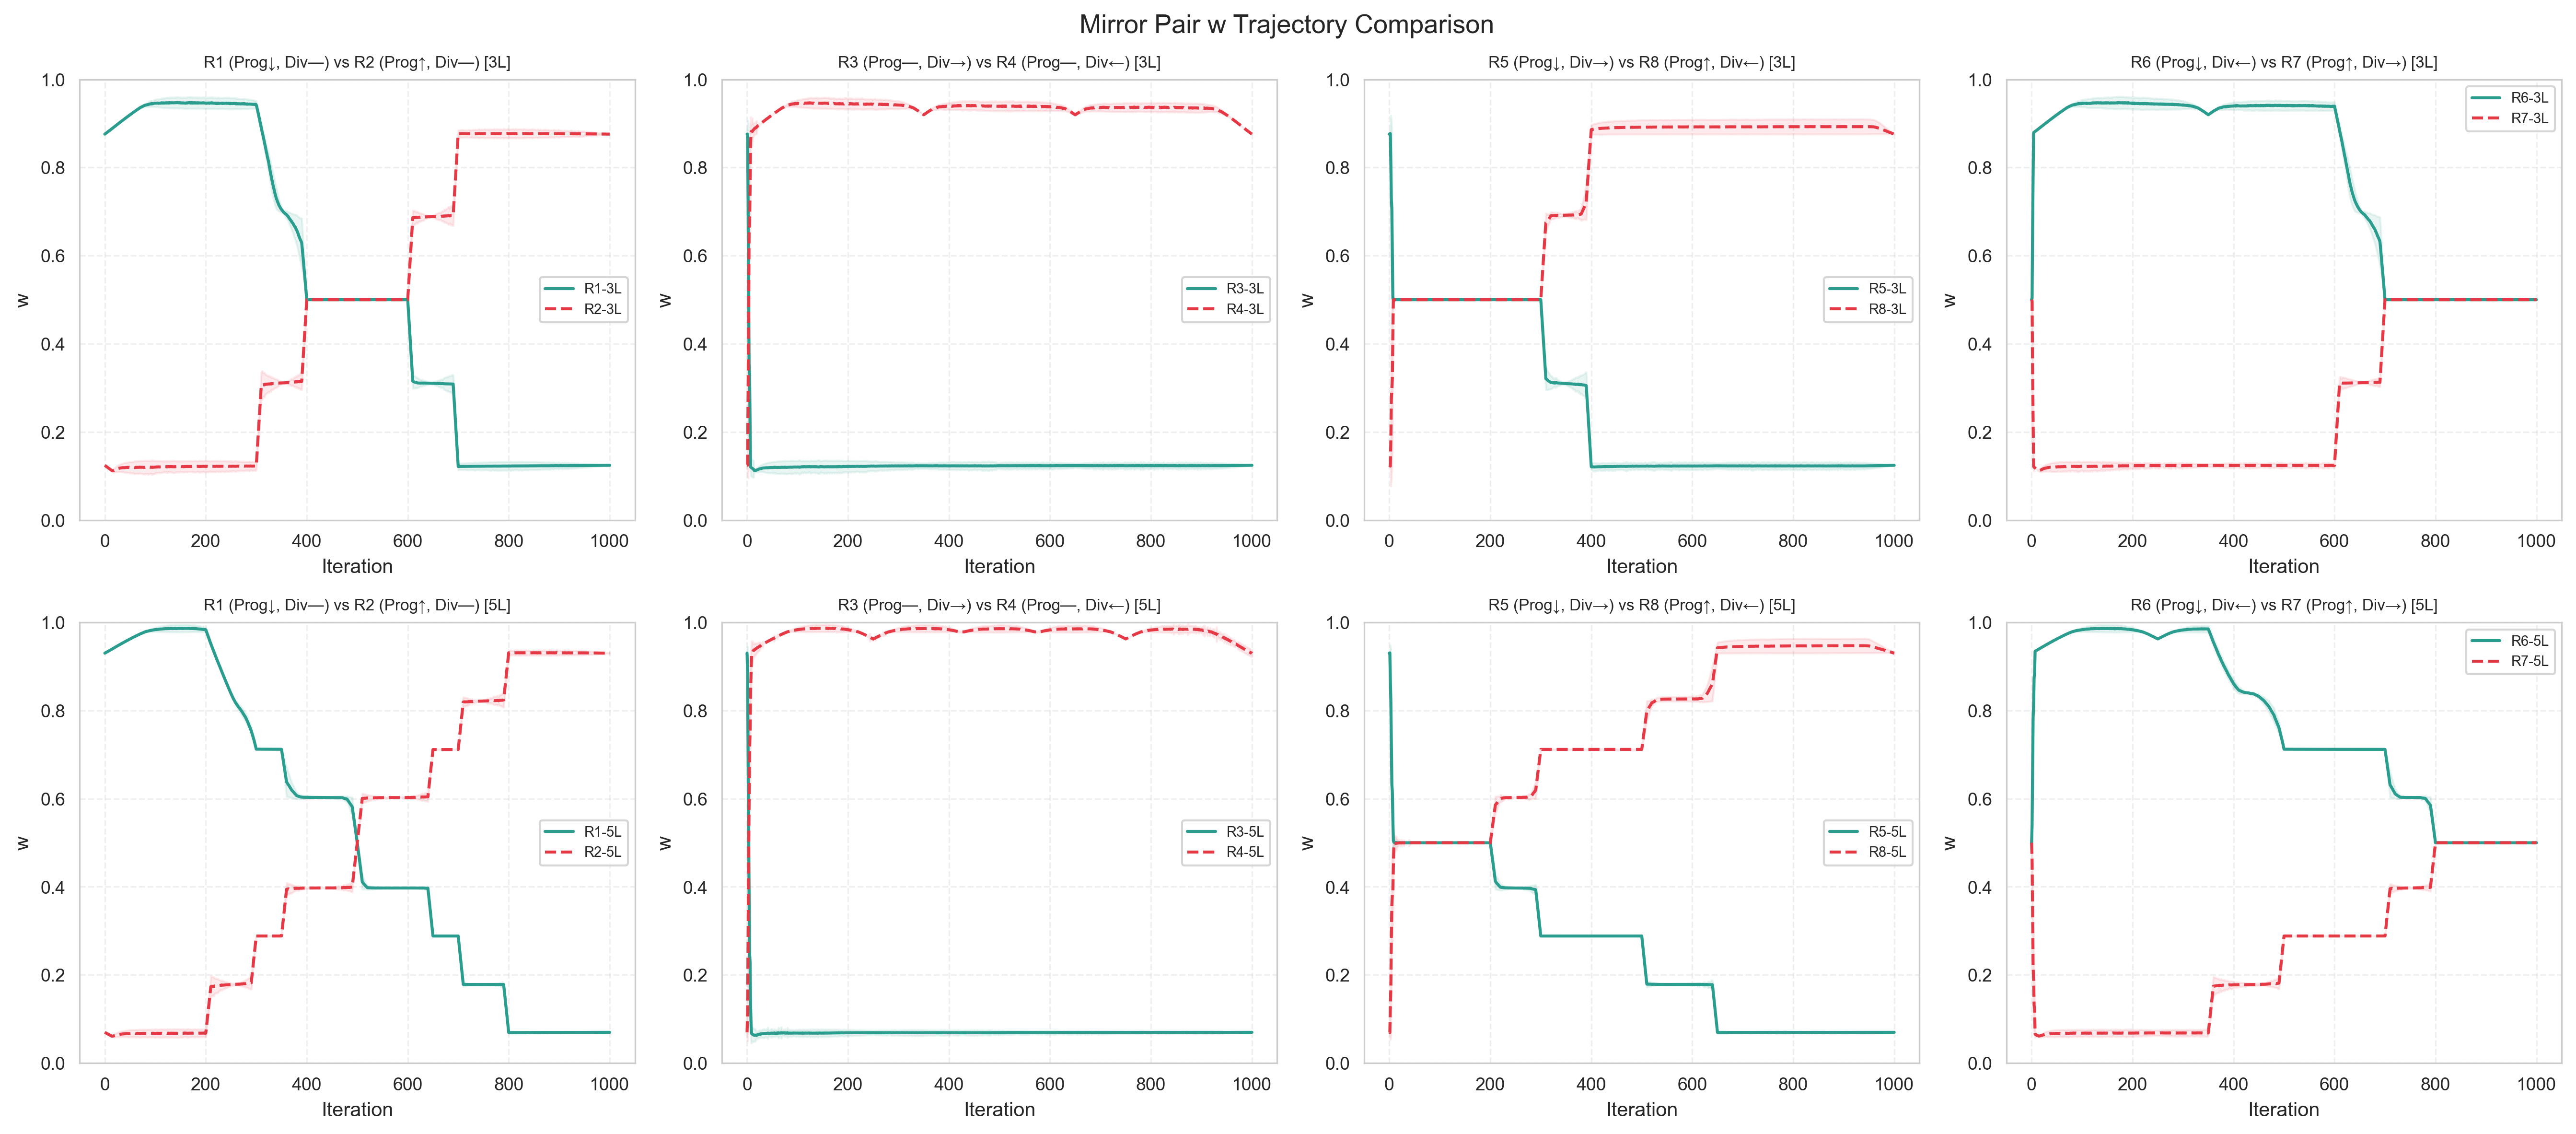
\includegraphics[width=0.95\textwidth]{resultados_wea/plots/05_mirror_pair_overlay.png}
\caption{Mean $w(t)$ trajectories for the four mirror pairs (rows: R1$\leftrightarrow$R2, R3$\leftrightarrow$R4, R5$\leftrightarrow$R8, R6$\leftrightarrow$R7) at 3L and 5L.}\label{fig:mirror}
\end{figure}

\vspace{-0.5cm}

The mechanistic origin is visible in Fig.~\ref{fig:mirror}: the four mirror pairs share the \emph{average} $w$-level but differ in how they distribute it across iterations. R1 (top-left) decreases $w$ from $0.9$ to $0.1$ along the progress axis, mirroring the linear PSO-STD ramp; its mirror R2 increases $w$ along the same axis. R3 follows the diversity signal and R4 compensates it; R5/R8 and R6/R7 correspond to the four sign combinations. Configurations that keep $w$ in the upper half of the range for most of the run (R2, R3, R7) cannot enter the exploitation phase and therefore stagnate orders of magnitude above the rest on F1, F5, F11; configurations whose $w$ trajectory descends to the $0.1$--$0.3$ band by the end of the run (R1, R5, R6, and PSO-STD) converge.



% ============================================================
\section{Conclusions and Future Work}\label{sec:conclusions}
% ============================================================


We analysed eight Mamdani rule bases under a controlled factorial design ($3{,}162$ runs, six benchmark functions, two granularities, all other FIS and PSO parameters fixed). Four observations stand out: (i)~progress direction is the dominant factor --- the mirror pair R1$\,\leftrightarrow\,$R2 yields the largest effect sizes ($|d|>3.5$, $p<10^{-11}$ on F1, F5, F11); (ii)~diversity reaction is a secondary, conditional contributor that helps when paired with a decreasing progress effect; (iii)~rule-base sensitivity concentrates in the optimum-zero, high-dimensional functions and is statistically inconclusive on the four-dimensional Shekel set; and (iv)~finer granularity amplifies rule quality in both directions --- refining R1 to the global winner (R1-5L) but worsening poorly oriented rule bases. The controller recovers, adaptively, a $w(t)$ profile close to the monotone-decreasing law of Shi and Eberhart when the correct progress trend is encoded into the rules.

These findings are subject to clear limitations: the benchmark covers only six functions of the F1--F23 suite, the input and output partitions are held at a single configuration each, only Mamdani min--max inference and COG defuzzification are tested, and PSO parameters are not co-tuned. Future work will (i)~extend the evaluation to the full F1--F23 set and to higher-dimensional and combinatorial benchmarks, (ii)~vary the input and output membership functions with the same factorial methodology applied here to the rule base, and (iii)~explore alternative inference operators (Sugeno, type-2 sets).

\begin{credits}
\subsubsection{\ackname}
José Barrera-García was supported by the National Agency for Research and Development ANID BECAS/DOCTORADO NACIONAL 21242516.
Felipe Cisternas-Caneo was supported by the National Agency for Research and Development ANID BECAS/DOCTORADO NACIONAL 21230203.
Broderick Crawford is supported by Grant ANID/FONDECYT/REGULAR/1262511.

%\subsubsection{\discintname}
%The authors have no competing interests to declare that are relevant to the content of this article.
\end{credits}
%
\bibliographystyle{splncs04}
\bibliography{references}
%
\end{document}

